
\documentclass[a4paper,UKenglish,cleveref, autoref]{lipics-v2019}
\usepackage{hyperref}
\usepackage{minted} % pip3 install pygments, pdflatex -shell-escape hb
\newminted[elpicode]{elpi.py:ElpiLexer -x}{linenos=true,fontsize=\footnotesize,escapeinside=\%\%}
\newmintinline[elpi]{elpi.py:ElpiLexer -x}{fontsize=\small}
\newminted[coqcode]{elpi.py:CoqElpiLexer -x}{linenos=true,fontsize=\footnotesize,mathescape,escapeinside=\#\#}
\newmintinline[coq]{elpi.py:CoqElpiLexer -x}{fontsize=\small}

\newcommand{\coqelpi}{Coq-Elpi}
\newcommand{\HB}{\ensuremath{\mathcal{HB}}}
\newcommand{\hb}{\coq{hierarchy-builder}}

%This is a template for producing LIPIcs articles. 
%See lipics-manual.pdf for further information.
%for A4 paper format use option "a4paper", for US-letter use option "letterpaper"
%for british hyphenation rules use option "UKenglish", for american hyphenation rules use option "USenglish"
%for section-numbered lemmas etc., use "numberwithinsect"
%for enabling cleveref support, use "cleveref"
%for enabling cleveref support, use "autoref"


%\graphicspath{{./graphics/}}%helpful if your graphic files are in another directory

\bibliographystyle{plainurl}% the mandatory bibstyle

\title{Hierarchy Builder: algebraic~hierarchies made easy in Coq with Elpi} %TODO Please add

\titlerunning{Hierarchy Builder}%optional, please use if title is longer than one line

\author{Cyril Cohen}{Inria, France}{Cyril.Cohen@inria.fr}{}{}
\author{Kazuhiko Sakaguchi}{University of Tsukuba, Japan}{sakaguchi@coins.tsukuba.ac.jp}{}{}
\author{Enrico Tassi}{Inria, France}{Enrico.Tassi@inria.fr}{}{}
\authorrunning{C.\,Cohen and K.\,Sakaguchi and E.\,Tassi}
% \author{John Q. Public}{Dummy University Computing Laboratory, [optional: Address], Country \and My second affiliation, Country \and \url{http://www.myhomepage.edu} }{johnqpublic@dummyuni.org}{https://orcid.org/0000-0002-1825-0097}{(Optional) author-specific funding acknowledgements}%TODO mandatory, please use full name; only 1 author per \author macro; first two parameters are mandatory, other parameters can be empty. Please provide at least the name of the affiliation and the country. The full address is optional
% \author{Joan R. Public\footnote{Optional footnote, e.g. to mark corresponding author}}{Department of Informatics, Dummy College, [optional: Address], Country}{joanrpublic@dummycollege.org}{[orcid]}{[funding]}
% \authorrunning{J.\,Q. Public and J.\,R. Public}%TODO mandatory. First: Use abbreviated first/middle names. Second (only in severe cases): Use first author plus 'et al.'

\Copyright{Cyril Cohen and Kazuhiko Sakaguchi and Enrico Tassi}%TODO mandatory, please use full first names. LIPIcs license is "CC-BY";  http://creativecommons.org/licenses/by/3.0/

\ccsdesc[100]{General and reference~General literature}
\ccsdesc[100]{General and reference}%TODO mandatory: Please choose ACM 2012 classifications from https://dl.acm.org/ccs/ccs_flat.cfm 
\supplement{Source code of the Coq package: \url{https://github.com/math-comp/hierarchy-builder}}
\keywords{Algebraic Hierarchy, Packed Classes, Coq, Elpi, Metaprogramming, $\lambda$Prolog}%TODO mandatory; please add comma-separated list of keywords

\category{}%optional, e.g. invited paper

\relatedversion{}%optional, e.g. full version hosted on arXiv, HAL, or other respository/website
%\relatedversion{A full version of the paper is available at \url{...}.}

\supplement{}%optional, e.g. related research data, source code, ... hosted on a repository like zenodo, figshare, GitHub, ...

%\funding{(Optional) general funding statement \dots}%optional, to capture a funding statement, which applies to all authors. Please enter author specific funding statements as fifth argument of the \author macro.

%\acknowledgements{I want to thank \dots}%optional

%\nolinenumbers %uncomment to disable line numbering

%\hideLIPIcs  %uncomment to remove references to LIPIcs series (logo, DOI, ...), e.g. when preparing a pre-final version to be uploaded to arXiv or another public repository

%Editor-only macros:: begin (do not touch as author)%%%%%%%%%%%%%%%%%%%%%%%%%%%%%%%%%%
\EventEditors{John Q. Open and Joan R. Access}
\EventNoEds{2}
\EventLongTitle{42nd Conference on Very Important Topics (CVIT 2016)}
\EventShortTitle{CVIT 2016}
\EventAcronym{CVIT}
\EventYear{2016}
\EventDate{December 24--27, 2016}
\EventLocation{Little Whinging, United Kingdom}
\EventLogo{}
\SeriesVolume{42}
\ArticleNo{23}
%%%%%%%%%%%%%%%%%%%%%%%%%%%%%%%%%%%%%%%%%%%%%%%%%%%%%%

\newcommand{\Lang}{\ensuremath{\Lambda}}
\newcommand{\term}{term}
\newcommand{\mixin}{primitive factory}
\newcommand{\mixins}{primitive factories}
\newcommand{\M}{\ensuremath{\mathcal{M}}}
\newcommand{\factory}{factory}
\newcommand{\factories}{factories}
\newcommand{\F}{\ensuremath{\mathcal{F}}}
\newcommand{\depx}{\ensuremath{d}}
\newcommand{\dep}{\ensuremath{dep}}
\newcommand{\depone}{\ensuremath{dep_1}}
\newcommand{\powerset}[1]{\raisebox{.15\baselineskip}{\Large\ensuremath{\wp}}(#1)}
\newcommand{\C}{\ensuremath{\mathcal{C}}}
\newcommand{\class}{class}
\newcommand{\classes}{classes}
\newcommand{\cdef}{\ensuremath{def}}
\newcommand{\Str}{\ensuremath{\mathcal{S}}}
\newcommand{\structure}{structure}
\newcommand{\structures}{structures}
\newcommand{\issubclass}{\ensuremath{sub}}
\newcommand{\subclass}{subclass}
\newcommand{\join}{\ensuremath{join}}
\newcommand{\requires}{\ensuremath{requires}}
\newcommand{\provides}{\ensuremath{provides}}
\newcommand{\from}{\ensuremath{\mathsf{from}}}
\newcommand{\proj}[2]{\ensuremath{#1[#2]}}
\newtheoremstyle{implem}{\topsep}{\topsep}{}{0pt}{\sffamily\bfseries}{ }{5pt plus 1pt minus 1pt}%
{$\blacktriangleright$ \thmname{#1}\thmnumber{ #2}\thmnote{ #3}}

\theoremstyle{implem}
\newtheorem*{implementation}{Implementation of}

\theoremstyle{implem}
\newtheorem*{invariant}{Programming invariant for}

\newcounter{axiomcounter}
\def\axiomcounterautorefname~#1\null{%
  Axiom~#1\null
}
\theoremstyle{axiom}
\newtheorem{axiom}[axiomcounter]{Axiom}

\newtheoremstyle{abscommand}{\topsep}{\topsep}{}{0pt}{\sffamily\bfseries}{ }{5pt plus 1pt minus 1pt}%
{$\blacktriangleright$ \thmname{#1}\coq{ #3}}
\theoremstyle{abscommand}
\newtheorem*{abscommand}{Command signature}

\newtheoremstyle{command}{\topsep}{\topsep}{}{0pt}{\sffamily\bfseries}{ }{5pt plus 1pt minus 1pt}%
{$\blacktriangleright$ \thmname{#1}\coq{ #3}}
\theoremstyle{command}
\newtheorem*{command}{Coq command}

\begin{document}

\maketitle

%TODO mandatory: add short abstract of the document
\begin{abstract}
It is nowadays customary to organize libraries of machine checked
proofs around hierarchies of algebraic
structures~\cite{10.1145/3372885.3373824,mathclasses,DBLP:journals/mics/BoldoLM15,DBLP:conf/mpc/AffeldtNS19}.
One influential example is the Mathematical Components library on top
of which the long and intricate proof of the Odd Order
Theorem could be fully formalized~\cite{DBLP:conf/itp/GonthierAABCGRMOBPRSTT13}.

Still, building algebraic hierarchies in a proof assistant such as Coq~\cite{Coq:manual}
requires a lot of manual labor and often a deep expertise in the internals of
the prover~\cite{DBLP:conf/tphol/GarillotGMR09,DBLP:conf/itp/MahboubiT13}.
Accommodating the evolution of a hierarchy, e.g
splitting a structure into two simpler ones, without causing breakage in
clint code is even harder, according to our experience~\cite{KSdraft}.

In this paper we describe \HB{}, a high level language
to \emph{build} hierarchies of algebraic structures and to make these hierarchies
\emph{evolve} without breaking user code. The key concept is the one of
\emph{\factory{}} that lets the hierarchy developer describe an actual
interface for his library. Behind that interface the developer can provide
appropriate code to ensure retro compatibility.
We implement the \HB{} language in the \hb{} addon for the Coq
system using the Elpi~\cite{DBLP:conf/lpar/DunchevGCT15,CoqElpi}
extension language.
\end{abstract}

%%%%%%%%%%%%%%%%%%%%%%%%%%%%%%%%%%%%%%%%%%%%%%%%%%%%%%%%%%%%%%%%%%%%%%%
\section{Introduction}
As of today The Mathematical Components library for the Coq system
provides the richest formal hierarchy of algebraic structures available:
groups, rings.... w/wo order, finite or countable, ...
The hierarcy is used to organize a large corpus of formal proofs and
is validate bu lange ones such as the 4CT and OOTHM.
The hierarchy is based on the discipline of Packed Classes initially introduced
in \cite{DBLP:conf/itp/GonthierAABCGRMOBPRSTT13} and later also used in
\cite{DBLP:conf/mpc/AffeldtNS19} and \cite{DBLP:journals/mics/BoldoLM15}
and MC analysis (paper? TR?)

We call Packed Classes a discpline, and not a language, because, in spite of
its many virtues, it is unwidly to use. In particular it leaks to the user
of the Coq system many of the technical details and compromises that were
needed in order to have it work reliably and efficiently. As as result one
needs to be an expert in order to master it, and even experts forget
to adhere to the discipline as shown in KS paper at CoqWS portland + TR?

Other approaches to declare hierarchies exist and were used in X y but
apparently failed to scale. Eg coquelicot stanted like that and then felt.

Moreover changes to an
already published hierarchy almost certainly break the code users.

In this paper we design a high level language for the Coq system to describe
hierarchies. We call this language \HB{}
This language introduces the notion of \emph{factory} that is key
to modify an existing hierarchy without breaking client code of the hierarchy.
The language is elaborated in terms of records, coercions and canonical
structure declarations, the same pillars on which packed classes stand on.
In order to simplify the elaboration
we chose to represent classes by simpler,
 \emph{flat}, records that regroup all the
axioms of the structure instead of nesting previously declared classes
into new ones.
We implement this language using the ELPI extension language for Coq.

%%%%%%%%%%%%%%%%%%%%%%%%%%%%%%%%%%%%%%%%%%%%%%%%%%%%%%%%%%%%%%%%%%%%%%%%5
\section{Example: building and evolving a hierarchy}

The first version of our hierarchy (that we name V1) features only two
structures: \coq{TYPE}, a naked carrier type without any properties, and
\coq{Ring}.

% TODO: remove TYPE, TYPE -> Type
% TOD: try TYPE -> Monoid

\begin{coqcode}
Elpi hb.structure TYPE.                            #\label{demo:structure:type}#

Elpi hb.declare_primitive_factory Ring_of_TYPE A.           #\label{demo:declare_primitive_factory:rot}#
  Record axioms := Axioms {
    zero : A;
    one : A;
    add : A -> A -> A;
    opp : A -> A;
    mul : A -> A -> A;
    addrA : associative add;             (* `add` is associative. *)
    addrC : commutative add;             (* `add` is commutative. *)
    add0r : left_id zero add;            (* `zero` is a (left) absorbing element *)
                                         (* w.r.t. `add`. *)
    addNr : left_inverse zero opp add;   (* `opp x` is the additive inverse of `x`. *)
    mulrA : associative mul;             (* `mul` is associative. *)
    mul1r : left_id one mul;             (* `one` is the left and right identity *)
    mulr1 : right_id one mul;            (* element w.r.t. `mul`. *)
    mulrDl : left_distributive mul add;  (* `mul` is left and right distributive over *)
    mulrDr : right_distributive mul add; (* `add`. *)
  }.
Elpi hb.end.                                #\label{demo:declare_primitive_factory:rot:end}#
Elpi hb.structure Ring Ring_of_TYPE.axioms.
\end{coqcode}

The \coq{hb.structure} command takes in input a name S and a possibly
empty list of assets. It registers a structure S in the hierarchy placing
any definition specific to that structure inside a Coq module named \coq{S}.
Line~\ref{demo:structure:type} hence forges a the empty structure \coq{TYPE}.

In order to build a non empty structure we need to declare some assets and
later assemble them. One kind of asset supported by \HB{} is called
\emph{mixin} and is embodied by a record, by convention named \coq{axioms},
that packs operations and properties.
Mixins are declared via the \coq{hb.declare_primitive_factory} command
that takes a module name,
a type variable name and a possibly empty list of assets for that type.
The code between lines~\ref{demo:declare_primitive_factory:rot}
and~\ref{demo:declare_primitive_factory:rot:end} declares a mixin that can turn a naked
type into a ring, hence we chose the module name to be \coq{Ring_of_TYPE}.

The last line declares the structure \coq{Ring} to hold the asset that
was just declared. We can now inspect the contents of the hierarchy and then
proceed to build a theory about abstract rings,
register examples (instances) of ring structures
and finally use the abstract theory on these examples.

\begin{coqcode}
Print Ring.type. (* Ring.type  :=  { sort : Type;  class : Ring.class_of sort } *) #\label{demo:theory:print:type}#
Check @add.      (* add        :   forall R : Ring.type, R -> R -> R            *) #\label{demo:theory:check:zero}#
Check @add0r.    (* add0r      :   forall R : Ring.type, left_id zero add       *) #\label{demo:theory:check:add0r}#

Lemma addr0 : forall R : Ring.type, right_id (@zero R) add. #\label{demo:theory:state:addr0}#
Proof. by move=> x; rewrite addrC add0r. Qed.

Definition Z_ring_axioms :=                               #\label{demo:theory:zaxioms}#
  Ring_of_TYPE.Axioms Z 0%Z 1%Z Z.add Z.opp Z.mul
    Z.add_assoc Z.add_comm Z.add_0_l Z.add_opp_diag_l
    Z.mul_assoc Z.mul_1_l Z.mul_1_r
    Z.mul_add_distr_r Z.mul_add_distr_l.

Elpi hb.canonical Z Z_ring_axioms.                        #\label{demo:theory:zaxioms:canonical}#

Lemma exercise (m n : Z) : - n + (n + m) + 0 = m.
Proof. rewrite addrA addNr add0r addr0. Qed.
\end{coqcode}

We can print the type for rings as forged by \HB{} (line~\ref{demo:theory:print:type}).
It packs a carrier, called \coq{sort}, and the collection of operation and
properties, called \coq{class}.  We can also look at the type of two
constants synthesized by \HB{} out of the hierarchy declaration. Remark that
while the names of the constants come from the the names of the mixin fields,
their types differ.
In particular they are quantified over a \coq{Ring.type}, and not
a simple type as in the mixin. Moreover we evince that
the \coq{sort} projection is declared as an implicit coercion~\cite{Saibi97} and is automatically
inserted in order to make \coq{R -> R -> R} a meaningful type for binary
operations on the carrier of \coq{R}.

We then prove lemma \coq{addr0}, line~\ref{demo:theory:state:addr0}, that is
a trivial consequence of the ring axioms. Albeit simple this example shows
we can populate the theory of rings with new results.

% TODO: packager: clarify the use of phantoms, not just a regular constructor
We use the \coq{Ring_of_TYPE.Axioms} \emph{packager} (line~\ref{demo:theory:zaxioms})
in order to build an instance of the \coq{Ring} structure for binary integers \coq{ZArith.BinInt.Z}.
We then register that ring instance as the canonical one on \coq{Z}
(line~\ref{demo:theory:zaxioms:canonical}).
From now on the theory of rings applies to
integers, as shown in lemma \coq{exercise}.
\marginpar{I use Axiom and not Axioms\_ everywhere, I think we should name
Axioms\_ the low level constructor, and Axioms the one with phantoms}.

\subsection{Evolution of the hierarchy}

We now proceed by changing the hierarchy to accomodate the intermediate
structure \coq{AddComoid} of additive commutative monoids.

\begin{coqcode}
Elpi hb.structure TYPE.

Elpi hb.declare_primitive_factory AddComoid_of_TYPE A.
  Record axioms := Axioms {
    zero : A;
    add : A -> A -> A;
    addrA : associative add;
    addrC : commutative add;
    add0r : left_id zero add;
  }.
Elpi hb.end.
Elpi hb.structure AddComoid AddComoid_of_TYPE.axioms.

Elpi hb.declare_primitive_factory Ring_of_AddComoid A AddComoid.class_of. #\label{demo2:mixin:ring}#
  Record axioms := Axioms {
    opp : A -> A;
    one : A;
    mul : A -> A -> A;
    addNr : left_inverse zero opp add;
    mulrA : associative mul;
    mul1r : left_id one mul;
    mulr1 : right_id one mul;
    mulrDl : left_distributive mul add;
    mulrDr : right_distributive mul add;
  }.
Elpi hb.end.
Elpi hb.structure Ring AddComoid_of_TYPE.axioms Ring_of_AddComoid.axioms. #\label{demo2:structure:ring}#
\end{coqcode}

The first interesting line is~\ref{demo2:mixin:ring} where we declare a mixin
for a type variable \coq{A}. This time \coq{A} is not a naked type, but rather
a type for which the the assets of a commutative monoid are available.
\marginpar{we did not show class\_of, it would be much nicer to have an axioms (from type) thing}
This is why the operation \coq{add} is in scope and can be used
together with new operations such as \coq{opp} to state properties, for
example \coq{addNr}.
We conclude by declaring the ring structure as the structure featuring both
mixins declared so far.

With this new version of the hierarchy, that we name V2, some code written
for version V1 breaks. For example the simple proof of \coq{addr0} works
but the declaration of the canonical ring over the integers fails, if only
because we don't have a \coq{Ring_of_TYPE.Axiom} packager anymore.

Our objective is to obtain a version of the hierarchy, say V3, that does
not only feature commutative monoids but that is also backward compatible
with V1.

% TODO: Write glossary
% remove distinction
% TODO: Structure -> Class
% TODO: packager -> ClassBuilder
% TODO: Builder -> Builder
% Factories ( primitive / general ) ; kill mixin
\begin{figure}[!h]
  \begin{center}
    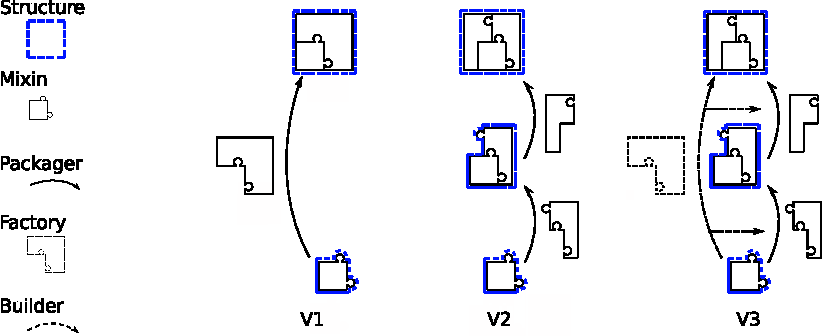
\includegraphics[width=\textwidth]{puzzle.pdf}
  \end{center}
  \caption{\label{fig:puzzle}The evolution of the hierarchy. V3 is backward compatible with V1, while V2 is not.}
\end{figure}

The key to make a hierarchy evolve without breaking user code is the second
kind of assets \HB{} provides: \emph{factories}.

Factories, like mixins, are packages for operations and properties but are
not directly used in the definition of structures. Instead a factory is
equipped with \emph{builders}: user provided pieces of code that extract
from the factory the contents of mixins, so that packagers can be used.

As depicted in figure~\ref{fig:puzzle} we change again the hierarchy
by declaring a \coq{Ring_of_TYPE} factory, that, from the user point of view,
will look indistinguishable from the old \coq{Ring_of_TYPE} mixin
and hence grant backward compatibility between this last version V3 and the
initial one V1.

\begin{coqcode}
Elpi hb.declare_factory Ring_of_TYPE A.
  Record axioms := Axioms {
    zero : A;
    one : A;
    add : A -> A -> A;
    opp : A -> A;
    mul : A -> A -> A;
    addrA : associative add;
    addrC : commutative add;
    add0r : left_id zero add;
    addNr : left_inverse zero opp add;
    mulrA : associative mul;
    mul1r : left_id one mul;
    mulr1 : right_id one mul;
    mulrDl : left_distributive mul add;
    mulrDr : right_distributive mul add;
  }.

  Variable f : axioms.                            #\label{demo3:variable:f}#

  Definition to_AddComoid_of_TYPE :=
    AddComoid_of_TYPE.Axioms A (zero f) (add f) (addrA f) (addrC f) (add0r f).
  Elpi hb.canonical A to_AddComoid_of_TYPE.

  Definition to_Ring_of_AddComoid :=
    Ring_of_AddComoid.Axioms A _ _ _ (addNr f) (mulrA f) (mul1r f) #\label{demo3:phantom}#
      (mulr1 f) (mulrDl f) (mulrDr f).
  Elpi hb.canonical A to_Ring_of_AddComoid.
Elpi hb.end.
\end{coqcode}

The record \coq{Ring_of_TYPE.axioms} is the same we declared as a mixin
in version V1. In order to make a factory out of it we equip it with
two constructions. The first is \coq{to_AddComoid_of_TYPE} and
explain how to build a \coq{AddComoid} structure out of the factory
axioms (named \coq{f}, line~\ref{demo3:variable:f}).
This construction is also registered as canonical for \coq{A},
so that the next construction \coq{to_Ring_of_AddComoid} can call
the \coq{Ring_of_AddComoid.Axioms} packager (that requires \coq{A} to be
an \coq{AddComoid} in order to fill in the three \coq{_} at
line~\ref{demo3:phantom}). In this simple example the two constructions are just
partitioning the contents of the factory \coq{f}, but in practice they
often involve interactive proofs that the properties held by the factory
imply the ones held by the mixins characterizing the structures that are
being constructed.

Once the factory is declared we can declare the \coq{Ring} structure
as we were doing in version V1, namely \coq{Elpi hb.structure Ring Ring_of_TYPE.axioms}.

Moreover we can declared \coq{Z} to be an instance
of a ring using the \coq{Ring_of_TYPE.axioms} factory.
The associated builder generats, behind the scenese, instances of the
\coq{Ring_of_AddComoid.axioms} and \coq{AddComoid_of_TYPE.axioms} mixins
that in turn are used to build instances of the \coq{AddComoid} and \coq{Ring}
structures. Indeed the command \coq{Elpi hb.canonical Z Z_ring_axioms}
makes \coq{Z} an instance of both structures.
Thanks to that the proof of \coq{example} can use the theory of
both structures, for example \coq{addr0} holds on rings, while \coq{addrA} holds
on commutative monoids. As a result the very same proof works on both
version V1 and V3.

%%%%%%%%%%%%%%%%%%%%%%%%%%%%%%%%%%%%%%%%%%%%%%%%%%%%%%%%%%%%%%%%%%%%%%%%
\section{An abstract presentation of \HB{}}

The user language of \HB{} is not tied to Coq and imposes very mild requirements
on the formal language to which it compiles to. We hence present \HB{} in an
abstracting setting.

\subsection{Preliminaries}

\begin{axiom}[\Lang{}, tagret language]\label{def:universe}
  \Lang{} is a set of names denoting terms of an target language.
  The language must feature projections. When
  a projection from $n$ to $m$ exists we write it \proj{n}{m}.
  The identity projection \proj{x}{x} always exists.
\end{axiom}

\begin{axiom}[(\M{}, \depx{}), \mixin{}]\label{def:mixin}
\( \M{} \subseteq \Lang{} \) is the finite set of \mixins{} and
\( \depx \in \M{} \to \powerset\M{} \) is a function expressing
dependencies among \mixins{}.
(\M{}, \depx{}) forms a Directed Acyclig Graph (DAG) and
\depx{} is transitively closed.
If \(m \in \depx{}(n) \) then \( \proj{n}{m} \in \Lang{} \)
\end{axiom}

\begin{definition}[\(\dep \in \powerset{\M{}} \to \powerset\M{}\)]\label{def:depxs}
\(
  \dep{}(M) = \bigcup_{m \in M} \depx (m)
\)
\end{definition}

\begin{definition}[\(\depone{} \in \M{} \to \powerset\M{}\)]\label{def:dep}
\(\depone{}(m) = \dep{}(\{m\})\)
\end{definition}

\begin{axiom}[(\C{}, \cdef{}), \class{}]\label{def:class}
\(\C{} \subseteq \Lang{}\) is the finite set of names for \classes{}.
\(\cdef{} \in \C \to \powerset\M{}\) is a function associating to
each \class{} a set of \mixins{}
such that \(\forall c \in \C{},~ \dep{}(\cdef{}(c)) \subseteq \cdef{}(c)\).
If \(m \in \cdef{}(c) \) then \( \proj{c}{m} \in \Lang{} \).
\cdef{} is injective (no two \classes{} contain the same set of \mixins{}).
\end{axiom}

\begin{axiom}[\Str{}, \structure{}]\label{def:structure}
\(\Str{} \subseteq \Lang{} \) is the finite set of names for \structures{}
and for each \class{} in \C{} there is one and only one \structure{}
in \Str{}.
\end{axiom}\marginpar{frankly, at this level of abstraction I don't see what
structures bring. Can't we talk about structures only when we package (in the
tgt lang?)}

\begin{axiom}[(\F{}, \requires{}, \provides{}, \from{}), \factory{}]\label{def:factory}
  \(\F{} \subseteq \Lang{} \) is the finite set of names for \factories{}.
  It is equipped with the three functions
  \begin{itemize}
    \item\( \requires{} \in \F{} \to \powerset\M{} \)
    \item\( \provides{} \in \F{} \to \powerset\M{} \)
    \item\( \from{} \in \F{} \times \M{} \to \Lang{} \)
  \end{itemize}
  that validate the following properties
  \begin{itemize}
    \item\( \forall f \in \F{},~ \dep{}(\requires{}(f)) \subseteq \requires{}(f)\)
    \item\( \forall f \in \F{},~ \requires{}(f) \cap \provides{}(f) = \emptyset \)
    \item\( \forall f \in \F{},~\exists c \in \C{},~ \cdef{}(c) = \requires{}(f) \cup \provides{}(f) \)
    \item\( \forall f \in \F{},~\exists C \subseteq \C{},~\bigcup_{c\in C}\cdef{}(c) = \requires{}(f)\)
    \item\( \forall f \in \F{},~\forall m \in \provides{}(f),~ \from{}(f,m) \) is defined
  \end{itemize}
\end{axiom}

\begin{proposition}[\( \M{} \subseteq \F{} \)]
  since \(\requires{}(m) = \depone{}(m)\)
  and \(\provides{}(m) = \{m\} \)
  and \(\from{}(m,m) = \proj{m}{m} \)
\end{proposition}

\begin{proposition}[\( \C{} \subseteq \F{} \)]
  since \(\requires{}(c) = \emptyset \)
  and \(\provides{}(c) = \cdef{}(c) \)
  and \(\from{}(c,m) = \proj{c}{m} \)
\end{proposition}

\subsection{extra}
THESE could be moved to the next subsection, since they don't help much here.
They only make sense after (or in) the chapter about Packed Classes, since
there you talk about joins.

\begin{definition}[\issubclass{} \(\in \C{}\times\C{}\), \subclass{}]\label{def:subclass}
\(c1~\issubclass{}~c2\) iff \(\cdef{}(c2) \subseteq \cdef{}(c1)\)
\end{definition}

\begin{definition}[\(\join{} \in \C{}\times\C{} \to \C{}\)]\label{def:join}
if \(c1, c2 \in \C{}\) and \(\cdef{}(c1) \cap \cdef{}(c2) \neq \emptyset\)
then \(\join{}(c1,c2)\) is the smallest \class{} \(c\) such that
\(\cdef{}(c1) \cup \cdef{}(c2) \subseteq \cdef{}(c)\).
\end{definition}

\begin{remark}[]
\(\join{}(c1,c2)\) is a \subclass{} of both \(c1\) and \(c2\).
\end{remark}

%%%%%%%%%%%%%%%%%%%%%%%%%%%%%%%%%%%%%%%%%%%%%%%%%%%%%%%%%%%%%%%%%%%%%%%%%%%%%
\subsection{The user language of \HB{}}

\begin{abscommand}[declare_primitive_factory] (fs : $\powerset\F{}$) (t : \Lang{}).\\
Declare a term t as a \mixin{}, adding it to \M{}, and defines
\( \dep{}(t) = \bigcup_{f \in fs} \requires{}(f) \).
\end{abscommand}

\begin{abscommand}[declare_factory] (fs : $\powerset\F{}$) (t : \Lang{}) (bs : $\powerset\Lang{}$).\\
Declare a term t as a \factory{}, adding it to \F{}, and defines
\begin{itemize}
\item \( \requires{}(t) = \bigcup_{f \in fs} \requires{}(f) \)
\item \( \provides{}(t) = HELP \)
\item \( \from{}(t,m) = b_m \)
\end{itemize}
\end{abscommand}

\begin{abscommand}[declare_structure] (fs : $\powerset\F{}$).\\
crafs a class $c \in \C{}$ where $\cdef{}(c) = HELP$ and its companion $s \in \Str{}$.
\end{abscommand}

\begin{abscommand}[instance] (c : $\Lang{}$) (fs : $\powerset\F{}$).\\
synthesizes terms in $\Lang{}$ corresponding to all the \mixins{} $MS$
that can be build with \from{} and all the \classes{} / \structures{}
for which \( \cdef{}(c) \subseteq MS \).
\end{abscommand}

When applied to a concrete \Lang{} the commands also take care of
accessory declarations, for example notations or inference directives.
In particular all operations of class c1 must be usable on c2 when
$c2~\issubclass{}~c1$, as well as points in c1 are also in c2.
The more these operations are implicit to the suser, the better.

For this reason we pick as a target language packed classes.

%%%%%%%%%%%%%%%%%%%%%%%%%%%%%%%%%%%%%%%%%%%%%%%%%%%%%%%%%%%%%%%%%%%%%%%%
\section{The target language: Coq with Packed, flat, Classes}
The language of packed classes were introduces in
\cite{DBLP:conf/tphol/GarillotGMR09} and used directly to describe the
algebraic hierarchy of the Mathematical Components library.
It is based on a disciplined use of records and projections and
on the possibility of extending the elaborator of Coq
via the declaration of Canonical Structures instances.

\subsection{Describing a structure with record and projections}

\begin{coqcode}
Module S.
  Record mixin A C := {
    one : A;
    op : A -> A -> A;
    opK : forall x, op (op x) = one
  }
  Record class_of A := {
    base : T.class_of A;
    mix  : mixin A base
  }.
  Record type := Pack {
    sort : Type;
    class : class_of sort
  }.
  Module Exports.
    Coercion sort : type >-> Sortclass.
    Definition op {T : type} : T -> T -> T := ...
    Definition one {T:  type} : T := ...
    Definition opK {T:  type} : forall x, op (op x) = one := ...
    Infix "*" := op.
    Infix "1" := one.
  End Exports.
End S.
\end{coqcode}

The module plays the role of a name space.
Export submodule is there because... I don't know.

\subsection{Linking structures and instances via Canonical Structures}

The mechanism of Canonical Structures~\cite{DBLP:conf/itp/MahboubiT13}
lets the user extend the elaborator of the Coq prover. This software component
takes in input a term as written by the user and has to infer all the missing
piece of information that is necessary to make the term well typed.

Example x + y * z

Here + and * come respectively from, but we are mising them, so we have
to find a common type that makes it work. This information comes from
the hierarchy and the links between the structures. The low level mechanism
is the unifier that compares p1 \_ = p2 \_ and has to find a common
superstructure...

The language lets us only write hints of the form p s = v, so we need two
of them here: (p1 s1 = p2 x) and (p1 y = p2 s2) for any x y.

Similarly one can apply an algebraic thoery to an instance (an example)
of a structure. Eg 1 * 2 + 3. The same mechanism of CS let us
extend the unifier to solve p1 \_ = nat.

\subsection{The flatten variant}

Describing a structure by proving a base class and a mixin is very conveniet
if one does it by hand, since it is more concise that spelling out all the
mixins by hand and is also closer to the user language one desires.

Since we are going to synthesize code automatically the have the freedom
to organize mixins as we wish while retaining a compact user language.
We chose to generate classes from scartch, listing all the involved
mixins since this more uniform.

TODO: Example of a by hand flatten class, maybe the one of the join.

%%%%%%%%%%%%%%%%%%%%%%%%%%%%%%%%%%%%%%%%%%%%%%%%%%%%%%%%%%%%%%%%%%%%%%%%%%%
\section{\HB{} in Coq}\label{sec:compilation}
this is the part of the readme that says "for each join declare a CS"

\begin{implementation}[\autoref{def:universe}]
We take the language of Coq as an implementation of \Lang{}.
\end{implementation}

\begin{implementation}[\autoref{def:mixin}]
A \mixin{} \coq{m} \(\in \M{}\) is a Coq record with one of more parameters.
The first parameter must be a \coq{(A : Type)}, while the other parameters are
are \mixins{} applied to \coq{A} and possibly other \mixins{}. E.g.
\begin{coqcode}
Record m3 (A : Type) (p1 : m1 A) (p2 : m2 A p1) := { ... }.
\end{coqcode}
for \coq{m1}, \coq{m2} and \coq{m3} \(\in \M{}\).
Given \(m \in \M{}\), \(\depx{}(m)\) is the set of all
\mixins{} that occur as parameters of \(m\), eg
\depx{}(\coq{m3}) = \{\coq{m2,m1}\} and \depx{}(\coq{m2}) = \{\coq{m1}\}.
\depx{} is transitively closed since records are well typed
in the empty context and describes a DAG since Coq does not
admit circular definitions.
Projections for parameters are trivially defineable.
In the packed classes lingo, this is a mixin.
\end{implementation}

\begin{implementation}[\autoref{def:class}]
A \class{} \coq{c} \(\in \C{}\) is a Coq record with with one parameter
\coq{(A : Type)}. The type of each field is a \mixin{} in \M{} applied to
\coq{A} and, if needed, any number of other fields. E.g.
\begin{coqcode}
Class c (A : Type) := { f1 : m1 A; ...; f3 : m3 A f1 f2; f4 : m2 A }.
\end{coqcode}
\(\cdef{}(c)\) is the set of \mixins{} mentioned in the fields of the \class{},
i.e. \{m1,m2,m3\}.
Given that \class{} records are well typed in the empty context
the set of \mixin{} records is closed transitively.
Projections for parameters are trivially defineable.
The implementation enforces that no two
\class{} records contains the same set of
\mixin{} (disregarding the order of the fields).
In the packed classeslingo, this is a flat class.
\end{implementation}

\begin{implementation}[\autoref{def:structure}]
A \structure{} \coq{s} \(\in \Str{}\) is a Coq record with with no parameters
and two fields. Its first field is \coq{(sort : Type)} and its second field is
\coq{(class : c sort)} for some \coq{c} \(\in \C{}\).
A structure is just a class closed with a sigma type on its parameter, hence
they are in bijection.
In the packed classes lingo, this is a structure.
\end{implementation}

\begin{implementation}[\autoref{def:factory}]
A \factory{} \coq{f} \(\in \F{}\) is a Coq record with one or more parameters.
The first parameter must be a \coq{(A : Type)}, while the other parameters are
are \factories{} (or \mixins) applied to \coq{A} and possibly other
\factories{} (or \mixins).

MORE
In the packed classes lingo, these are packagers.
\end{implementation}

\begin{command}[hb.declare_primitive_factory M A FS R := { .. } ]
registers in a db R...
\end{command}
\begin{command}[hb.declare_factory M A FS R := {... }. bs hb.end]
we split into two since the bs are hand and can be done interactively.
populates the context with...
the user labels the bs via isntance.
\end{command}
\begin{command}[hb.declare_structure]
declares many records/modules/coercions, for each join... exports operations,
theory submodule....
\end{command}
\begin{command}[hb.instance]
very close to the abstract one, but instruments CS inference with
the synthesizedterms.
\end{command}


%%%%%%%%%%%%%%%%%%%%%%%%%%%%%%%%%%%%%%%%%%%%%%%%%%%%%%%%%%%%%%%%%%%%%%%%%%%%
\section{The implementation in Coq-Elpi}\label{sec:implementation}

The implementation is based on the Elpi
extension language for Coq. In this section we introduce the features of the
programming language that came handy in the development of \HB{} and
commenting a few code snippets.

Coq-Elpi~\cite{CoqElpi} is a Coq plugin embedding
Elpi and providing an
extensive, high level, API to access and script the Coq system at the
vernacular level.
This API lives in the \elpi{coq.} namespace and lets one easily declare
records, coercions, canonical structures, modules, implicit arguments, etc.
The most basic Coq data type exposed to Elpi is the one of references to global
declarations:

\begin{elpicode}
kind gref  type.
type indt  inductive -> gref.    % eg: Coq.Init.Datatypes.nat
type indc  constructor -> gref.  % eg: Coq.Init.Datatypes.O
type const constant -> gref.     % eg: Coq.Init.Peano.plus
\end{elpicode}

The arguments of the three constructors are opaque to Elpi, that can only use
values of these types via dedicated APIs. For example the API for declaring
an inductive type will generate a value of type \elpi{inductive} that
would be printed as, for example, \elpi{«nat»}.

Elpi~\cite{DBLP:conf/lpar/DunchevGCT15} is a dialect
of $\lambda$Prolog~\cite{Miller:2012:PHL:2331097}, an higher order
logic programming language that makes it easy to manipulate abstract syntax
tree with binders. Coq-Elpi takes full adavantage of this capability by
representing Coq terms in HOAS style, reusing the binder of the programming
language in order to reprent Coq's ones. Here an excerpt of the data
type of Coq terms:

\begin{elpicode}
kind term type.
type global gref -> term.                    % eg: nat, O, S, plus, ...
type fun    term -> (term -> term) -> term.  % eg: fun x : t => b(x)
type app    list term -> term.               % eg: app [hd|args]
... % all other term constructors are omitted for brevity
\end{elpicode}

Notice that the \elpi{fun} constructor holds $\lambda$Prolog function.
In this syntax the Coq term \coq{(fun x : nat => x x)} becomes
\elpi{(fun (global (indt «nat»)) x\ app[x, x])} where \elpi{x\} binds \elpi{x}
in the body of the function. Substitution of a bound variable for a term
can be computed by applying a term (of function type) to an argument.

Data types with binders are also used as input to high level APIs that build
terms behind the scenes. For example a Coq record is just an inductive type
and the API do declare one must allow the type of a field to depend on the
fields that comes before it. Notice that the \elpi{field} constructor
takes a coercion flag, the name of the field, its type and binds a term
in the remaining record declaration.

\begin{elpicode}
kind indt-decl type.
type record      string -> term -> string -> record-decl -> indt-decl.
type field       bool -> string -> term -> (term -> record-decl) -> record-decl.
type end-record  record-decl.
... % constructors for non-record inductive types are omitted for brevity

external pred coq.env.add-indt i:indt-decl, o:inductive.
external pred coq.CS.canonical-projections i:inductive, o:list (option constant).
\end{elpicode}

The \elpi{pred} keyword documents a the type and modes (input or output) of the
arguments of a predicate, while \elpi{external} signals that the
predicate is a builtin (in other words it is implemented in
OCaml rather than $\lambda$Prolog).

We comment these two builtin predicates and the \elpi{indt-decl} type
while looking at the code of \elpi{declare-structure} that is in charge
of scripting the following Coq code (given as a parameter \coq{class_of}):

\begin{coqcode}
Record type : Type := Pack { sort : Type; class : class_of sort }.
\end{coqcode}

The Elpi code builds the declaration, typechecks it, adds it to the
Coq environment and returns the projections for the sort and the class
fields (it is handy to have them in the rest of the code).
TODO: factoryname -> @classname

\begin{elpicode}
pred declare-structure i:factoryname, o:term, o:term, o:term.

declare-structure ClassName Structure SortProjection ClassProjection :- std.do! [
  StructureDeclaration =
    record "type" {{ Type }} "Pack" (
      field ff "sort" {{ Type }} s\                        %\label{binder:sort}%
      field ff "class" (app [global ClassName, s]) _\
    end-record),
  coq.typecheck-indt-decl StructureDeclaration,
  coq.env.add-indt StructureDeclaration StructureName,     %\label{record:decl}%
  coq.CS.canonical-projections StructureName [some SortP, some ClassP],
  Structure = global (indt StructureName),
  SortProjection = global (const SortP),
  ClassProjection = global (const ClassP),
].
\end{elpicode}

Note that the binder \elpi{s\} at line \ref{binder:sort} lets one mention
the first field in the type of the second.
The syntax \elpi{{{ Type }}} is a quotation: it lets
one use the sytnax of Coq to write an Elpi expression of type \elpi{term}.
The API \elpi{coq.CS.canonical-projection} lets us find the projections
automatically generated by Coq for a given record.
The last detail worth discussing is that this program makes no use of
backtraking: the \elpi{std.do!} combinator signals that.

In the simple case of the structure record the number of fields, and hence
the number of binders, is fixed. On the contrary the class record has one
field per mixin and each of them can depend on the previous ones.
In order to synthesize terms with binders in an inductive fashion (using
a recursive predicate) $\lambda$Prolog lets one postulate fresh nominal
constants using the \elpi{pi} operator and attach to the
nominal some knowledge in the form of a clause via the \elpi{=>} operator.
This process is called binder mobility: the binder is moved from
the data (that we are bilding) to the program (the context of the
current computation).
This feature is key to in the following code that synthesizes the
declaration of the fields of the class record.

\begin{elpicode}
pred synthesize-fields.field-for-mixin i:mixinname, o:term.
pred synthesize-fields i:list mixinname, i:term, o:record-decl.

synthesize-fields [] _ Decl :- Decl = end-record.
synthesize-fields [M|ML] T Decl :- std.do! [
  get-mixin-modname M ModName,
  Name is ModName ^ "_mixin",                          %\label{craft:name}%
  dep1 M Deps,                                         %\label{deps:fetch}%
  std.map Deps synthesize-fields.field-for-mixin Args, %\label{deps:satisfy}%
  Type = app[ global M, T | Args ],                    %\label{build:type}%
  Decl = (field ff Name Type f\
          Fields f),
  pi m\                                                %\label{postulate:m}%
    synthesize-fields.field-for-mixin M m =>           %\label{postulate:satisfy}%
    synthesize-fields ML T (Fields m)                  %\label{rec:call}%
].
\end{elpicode}

The first predicate \elpi{synthesize-fields.field-for-mixin} is used
to link a mixin to a nominal that corresponds to the record field
for that mixin. It has no clauses in the base program but some clauses
are added dynamically by \elpi{synthesize-fields}.

The second predicate recurses on the (topologically sorted) list of mixins,
and terminates when the list is empty. If the list contains a mixin \elpi{M}
then it crafts a name for it \elpi{Name} (line \ref{craft:name}),
fetches its dependencies (line \ref{deps:fetch}) and
finds the (previous declared) record fields hoding these mixins
(line \ref{deps:satisfy}).
The \elpi{(std.map L1 P L2)} predicate relates the two lists \elpi{L1} and
\elpi{L2} pointwise using the predicate \elpi{P}.

Line \ref{build:type} builds the type of the field: the mixin name applied
to the type (sort) and all its dependencies.
Notice that the \elpi{Fields} variable, representing the declaration of the
next fields, is under the binder for \elpi{f} (the current field).
In order to recurse under that binder (line \ref{rec:call})
and recursively process \elpi{ML} we postulate a nominal
\elpi{m} (line \ref{postulate:m}) that is a term satisfying any
future dependency on the current mixin (line \ref{postulate:satisfy})
and we replace \elpi{f} by \elpi{m} in \elpi{Fields} by writing
\elpi{(Fields m)}.

The code of \elpi{synthesize-fields} makes an idiomatic use
of \elpi{=>} in $\lambda$Prolog: the current program is temporarily
extended with a clause. The same operation, but with a persistent
effect, is made available by Coq-Elpi via a dedicated API to extend
data bases. A data base is a named set of clauses and
commands are typically built by accumulating specific clauses on top
of a data base. Here an excerpt of the \verb+hierarchy.db+ data base and
of the \elpi{declare_primitive_factory} command. Text between \verb+lp:{{+ and \verb+}}+
is Elpi code embedded in a Coq file. All the vernacular commands beginning
with \coq{Elpi} are provided by the Coq-Elpi plugin.

\begin{coqcode}
Elpi Db hierarchy.db lp:{{
  pred dep1 o:mixinname, o:list mixinname.
  ... % for brevity we omit class and join
}}.
Elpi Command declare_primitive_factory.
Elpi Accumulate Db hierarchy.db.
Elpi Accumulate lp:{{
  main [str S] :- !, std.do! [
    coq.locate S M,
    coq.env.typeof M Ty,
    gather-mixin-dendencies Ty [] ML, % implementation omitted for brevity
    coq.elpi.accumulate "hierarchy.db" (clause _ _ (dep1 M ML)),
    ...
  ].
  main _ :- coq.error "Usage: declare_primitive_factory <mixin>".
}}.
\end{coqcode}

Line 11 computes the dependencies of mixin \elpi{M} given
its type and line 12 crafs a clause for \elpi{dep1} and
adds it to the data base \elpi{"hierarchy.db"}.

%%%%%%%%%%%%%%%%%%%%%%%%%%%%%%%%%%%%%%%%%%%%%%%%%%%%%%%%%%%%%%%%%%%%%%%%%%%%%
%\section{Benchmark}
%if we can port ssralg, or not... It would be nice, but maybe its a bit late.

%%%%%%%%%%%%%%%%%%%%%%%%%%%%%%%%%%%%%%%%%%%%%%%%%%%%%%%%%%%%%%%%%%%%%%%%%%%%%
\section{Related work}
The closest work is the one about Packed Classes~\cite{DBLP:conf/tphol/GarillotGMR09} on which we
build. The main differences are that \HB{} is a higher level language
that is compiled down to Flat Packed Classes. The systematic use of
factories makes the user interface of a hierarchy stable under the insertion of
intermediate structures in the hierarchy, a property that Packed Classes lacks.
Finally many of the intricacy of Packed Classes are hidden to the user by
the compilation step, making the language less error prone.
\marginpar{ET: I guess you have more to say here}

In~\cite{CaretteCombinators} Carette and O'Connor describe the language of
Theory Presentation Combinators that can be used to describe a hierarchy of
algebraic structures.
They focus on the categorical semantics of the language that is built upon
the category of context.
They don't describe any actual compilation to the language of a mainstream
interactive prover, indeed they claim their language to be mostly type theory
independent. We know they considered targeting type theory and the language
of unification hints~\cite{10.1007/978-3-642-03359-9_8}
(a superset of the one of Canonical Structures),
but we could not find any written trace of that. Language wise they provides
keywords such as \verb+combine+ and \verb+over+ to share (reuse) a property
when defining a new structure. For example in order to avoid restating
the commutativity property when defining abelian groups they combine
a commutative monoid and a group focing the subjacent monoid to coincide:
\begin{verbatim}
CommutativeGroup := combine CommutativeMonoid , Group over Monoid
\end{verbatim}
In our language \HB{} the same role is played by \emph{mixins}.
A mixin lets one write once and forall a property and abstract it over types
and operations so that it can be reused in all the structures that need it.
TODO: cyril fix this sentence

The MMT system~\cite{RABE20131} provides a framework to describe formal
languages in a logical framework, providing good support for binders and
notations. It also provides an expressive module system to organize
theories and express relations among them in the form of functors.
At the time of writing
it provides limited support for elaborating user input taking systematic
advantage of the contents of the theories. The elborator can be extended
by the user writing Scala code, and in principle use the contents of the
libraries to make sense of an incomplete expressions, but no higher level
language or mechanism is provided.

The library of the Mizar system features a hierarchy of algebraic
structures~\cite{7733265}. In spite of lacking dependent types, Mizar
provides the concept of attributed types and adjectives
that can be used to describe he signature of structures as one would
do with a dependently typed record and their properties as
one would define a conjunctive predicate.
The Mizar language also provides the notation of cluster that is used
to link structures: by showing that property $P$ implies property $Q$
one can inform automation that structures characterized by $P$ are
instances of structures characterized by $Q$. The foundational theory of Mizar
is characterized by an extensional notion of equality that makes it easy
to share the signature or the properties of structures by just requiring
a proof of their equivalence that is in turn used by autmation to treat
equivalent structures as equal.

TODO: the word factory comes from "the gang of four" design patterns, we
could cite it. Cyril sees a similarity between the AbstractFactory design
pattern and our notion of factory.

\subsection{Other target languages}

We could have chosen nested records (pollack) or unbundled (spitters)
but both have serious performance issue, the latter partially mitigated by
the addition of primitive records. TC implementation in Coq is not as
reliable as CS.

It is a virtue of our work to provide a user language that is separate
from the implementation one, so we could in principle target any other
equally expressive language without the user noticing.

%%%%%%%%%%%%%%%%%%%%%%%%%%%%%%%%%%%%%%%%%%%%%%%%%%%%%%%%%%%%%%%%%%%%%%%%%%%%
\section{Conclusion}
In this paper we design and implement \HB{}, a high level language to describe
hierarchies of algebraic structures. The implementation of \HB{} is
based on the Elpi excension language for the Coq system and is available
at \url{https://github.com/math-comp/hierarchy-builder}.

The high level language is not tied to Coq or even Type Theory.
It could hence be adopt without major changes in other tools. Indeed the
properties and invariants that link \factories{}, \mixins{} and \classes{}
are key to rule out meaningless or ambiguous sentences and are not
specific to the logic setting on which a prover stands.

The compilation scheme we present in section \ref{sec:compilation} is of
course tied to dependent records
and Canonical Structures, features that are tied to Coq but also available
in other provers based on Type Theory such a Matita and Lean that provide
unification hints, a strict superlanguage of Canonical Structures.

We leave to future work:
\begin{itemize}
\item derive the type/definition of morphisms between structures part of the
      hierarchy, this requires assuming more on \Lang{} (eg operations,
      equality)
\item support structures indexed by other structures, eg modules over as ring.
      SAY MORE, hintat the fact that these indexes must be organized in a
      hierarchy themselves
\end{itemize}

%The implementation presented in section \ref{sec:implementation} is tied
%to the Coq-Elpi plugin, which provides both the Elpi language and a comprehensive
%set of APIs. While the APIs are tied to Coq, the Elpi programming language
%comes as an OCaml library and could, in principle, be linked to other provers.

\bibliography{biblio}

\appendix

\section{Coq reference}

\begin{coqcode}
Section OperationProperties.
Variable T : Type.
Variable e : T.
Variable inv : T -> T.
Variable op : T -> T -> T.
Variable add : T -> T -> T.

Definition left_id  := forall x, op e x = x.
Definition right_id := forall x, op x e = x.

Definition left_inverse := forall x, op (inv x) x = e.

Definition commutative := forall x y, op x y = op y x.
Definition associative := forall x y z, op x (op y z) = op (op x y) z.

Definition left_distributive  := forall x y z, op (add x y) z = add (op x z) (op y z).
Definition right_distributive := forall x y z, op x (add y z) = add (op x y) (op x z).
\end{coqcode}

\end{document}



\section{Typesetting instructions -- Summary}
\label{sec:typesetting-summary}

LIPIcs is a series of open access high-quality conference proceedings across all fields in informatics established in cooperation with Schloss Dagstuhl. 
In order to do justice to the high scientific quality of the conferences that publish their proceedings in the LIPIcs series, which is ensured by the thorough review process of the respective events, we believe that LIPIcs proceedings must have an attractive and consistent layout matching the standard of the series.
Moreover, the quality of the metadata, the typesetting and the layout must also meet the requirements of other external parties such as indexing service, DOI registry, funding agencies, among others. The guidelines contained in this document serve as the baseline for the authors, editors, and the publisher to create documents that meet as many different requirements as possible. 

Please comply with the following instructions when preparing your article for a LIPIcs proceedings volume. 
\paragraph*{Minimum requirements}

\begin{itemize}
\item Use pdflatex and an up-to-date \LaTeX{} system.
\item Use further \LaTeX{} packages and custom made macros carefully and only if required.
\item Use the provided sectioning macros: \verb+\section+, \verb+\subsection+, \verb+\subsubsection+, \linebreak \verb+\paragraph+, \verb+\paragraph*+, and \verb+\subparagraph*+.
\item Provide suitable graphics of at least 300dpi (preferably in PDF format).
\item Use BibTeX and keep the standard style (\verb+plainurl+) for the bibliography.
\item Please try to keep the warnings log as small as possible. Avoid overfull \verb+\hboxes+ and any kind of warnings/errors with the referenced BibTeX entries.
\item Use a spellchecker to correct typos.
\end{itemize}

\paragraph*{Mandatory metadata macros}
Please set the values of the metadata macros carefully since the information parsed from these macros will be passed to publication servers, catalogues and search engines.
Avoid placing macros inside the metadata macros. The following metadata macros/environments are mandatory:
\begin{itemize}
\item \verb+\title+ and, in case of long titles, \verb+\titlerunning+.
\item \verb+\author+, one for each author, even if two or more authors have the same affiliation.
\item \verb+\authorrunning+ and \verb+\Copyright+ (concatenated author names)\\
The \verb+\author+ macros and the \verb+\Copyright+ macro should contain full author names (especially with regard to the first name), while \verb+\authorrunning+ should contain abbreviated first names.
\item \verb+\ccsdesc+ (ACM classification, see \url{https://www.acm.org/publications/class-2012}).
\item \verb+\keywords+ (a comma-separated list of keywords).
\item \verb+\relatedversion+ (if there is a related version, typically the ``full version''); please make sure to provide a persistent URL, e.\,g., at arXiv.
\item \verb+\begin{abstract}...\end{abstract}+ .
\end{itemize}

\paragraph*{Please do not \ldots} %Do not override the \texttt{\seriesstyle}-defaults}
Generally speaking, please do not override the \texttt{lipics-v2019}-style defaults. To be more specific, a short checklist also used by Dagstuhl Publishing during the final typesetting is given below.
In case of \textbf{non-compliance} with these rules Dagstuhl Publishing will remove the corresponding parts of \LaTeX{} code and \textbf{replace it with the \texttt{lipics-v2019} defaults}. In serious cases, we may reject the LaTeX-source and expect the corresponding author to revise the relevant parts.
\begin{itemize}
\item Do not use a different main font. (For example, the \texttt{times} package is forbidden.)
\item Do not alter the spacing of the \texttt{lipics-v2019.cls} style file.
\item Do not use \verb+enumitem+ and \verb+paralist+. (The \texttt{enumerate} package is preloaded, so you can use
 \verb+\begin{enumerate}[(a)]+ or the like.)
\item Do not use ``self-made'' sectioning commands (e.\,g., \verb+\noindent{\bf My+ \verb+Paragraph}+).
\item Do not hide large text blocks using comments or \verb+\iffalse+ $\ldots$ \verb+\fi+ constructions. 
\item Do not use conditional structures to include/exclude content. Instead, please provide only the content that should be published -- in one file -- and nothing else.
\item Do not wrap figures and tables with text. In particular, the package \texttt{wrapfig} is not supported.
\item Do not change the bibliography style. In particular, do not use author-year citations. (The
\texttt{natbib} package is not supported.)
\end{itemize}

\enlargethispage{\baselineskip}

This is only a summary containing the most relevant details. Please read the complete document ``LIPIcs: Instructions for Authors and the \texttt{lipics-v2019} Class'' for all details and don't hesitate to contact Dagstuhl Publishing (\url{mailto:publishing@dagstuhl.de}) in case of questions or comments:
\href{http://drops.dagstuhl.de/styles/lipics-v2019/lipics-v2019-authors/lipics-v2019-authors-guidelines.pdf}{\texttt{http://drops.dagstuhl.de/styles/lipics-v2019/\newline lipics-v2019-authors/lipics-v2019-authors-guidelines.pdf}}

\section{Lorem ipsum dolor sit amet}

Lorem ipsum dolor sit amet, consectetur adipiscing elit \cite{DBLP:journals/cacm/Knuth74}. Praesent convallis orci arcu, eu mollis dolor. Aliquam eleifend suscipit lacinia. Maecenas quam mi, porta ut lacinia sed, convallis ac dui. Lorem ipsum dolor sit amet, consectetur adipiscing elit. Suspendisse potenti. Donec eget odio et magna ullamcorper vehicula ut vitae libero. Maecenas lectus nulla, auctor nec varius ac, ultricies et turpis. Pellentesque id ante erat. In hac habitasse platea dictumst. Curabitur a scelerisque odio. Pellentesque elit risus, posuere quis elementum at, pellentesque ut diam. Quisque aliquam libero id mi imperdiet quis convallis turpis eleifend. 

\begin{lemma}[Lorem ipsum]
\label{lemma:lorem}
Vestibulum sodales dolor et dui cursus iaculis. Nullam ullamcorper purus vel turpis lobortis eu tempus lorem semper. Proin facilisis gravida rutrum. Etiam sed sollicitudin lorem. Proin pellentesque risus at elit hendrerit pharetra. Integer at turpis varius libero rhoncus fermentum vitae vitae metus.
\end{lemma}

\begin{proof}
Cras purus lorem, pulvinar et fermentum sagittis, suscipit quis magna.

\begin{claim}
content...
\end{claim}
\begin{claimproof}
content...
\end{claimproof}

\end{proof}

\begin{corollary}[Curabitur pulvinar, \cite{DBLP:books/mk/GrayR93}]
\label{lemma:curabitur}
Nam liber tempor cum soluta nobis eleifend option congue nihil imperdiet doming id quod mazim placerat facer possim assum. Lorem ipsum dolor sit amet, consectetuer adipiscing elit, sed diam nonummy nibh euismod tincidunt ut laoreet dolore magna aliquam erat volutpat.
\end{corollary}

\begin{proposition}\label{prop1}
This is a proposition
\end{proposition}

\autoref{prop1} and \cref{prop1} \ldots

\subsection{Curabitur dictum felis id sapien}

Curabitur dictum \cref{lemma:curabitur} felis id sapien \autoref{lemma:curabitur} mollis ut venenatis tortor feugiat. Curabitur sed velit diam. Integer aliquam, nunc ac egestas lacinia, nibh est vehicula nibh, ac auctor velit tellus non arcu. Vestibulum lacinia ipsum vitae nisi ultrices eget gravida turpis laoreet. Duis rutrum dapibus ornare. Nulla vehicula vulputate iaculis. Proin a consequat neque. Donec ut rutrum urna. Morbi scelerisque turpis sed elit sagittis eu scelerisque quam condimentum. Pellentesque habitant morbi tristique senectus et netus et malesuada fames ac turpis egestas. Aenean nec faucibus leo. Cras ut nisl odio, non tincidunt lorem. Integer purus ligula, venenatis et convallis lacinia, scelerisque at erat. Fusce risus libero, convallis at fermentum in, dignissim sed sem. Ut dapibus orci vitae nisl viverra nec adipiscing tortor condimentum \cite{DBLP:journals/cacm/Dijkstra68a}. Donec non suscipit lorem. Nam sit amet enim vitae nisl accumsan pretium. 

\begin{lstlisting}[caption={Useless code},label=list:8-6,captionpos=t,float,abovecaptionskip=-\medskipamount]
for i:=maxint to 0 do 
begin 
    j:=square(root(i));
end;
\end{lstlisting}

\subsection{Proin ac fermentum augue}

Proin ac fermentum augue. Nullam bibendum enim sollicitudin tellus egestas lacinia euismod orci mollis. Nulla facilisi. Vivamus volutpat venenatis sapien, vitae feugiat arcu fringilla ac. Mauris sapien tortor, sagittis eget auctor at, vulputate pharetra magna. Sed congue, dui nec vulputate convallis, sem nunc adipiscing dui, vel venenatis mauris sem in dui. Praesent a pretium quam. Mauris non mauris sit amet eros rutrum aliquam id ut sapien. Nulla aliquet fringilla sagittis. Pellentesque eu metus posuere nunc tincidunt dignissim in tempor dolor. Nulla cursus aliquet enim. Cras sapien risus, accumsan eu cursus ut, commodo vel velit. Praesent aliquet consectetur ligula, vitae iaculis ligula interdum vel. Integer faucibus faucibus felis. 

\begin{itemize}
\item Ut vitae diam augue. 
\item Integer lacus ante, pellentesque sed sollicitudin et, pulvinar adipiscing sem. 
\item Maecenas facilisis, leo quis tincidunt egestas, magna ipsum condimentum orci, vitae facilisis nibh turpis et elit. 
\end{itemize}

\begin{remark}
content...
\end{remark}

\section{Pellentesque quis tortor}

Nec urna malesuada sollicitudin. Nulla facilisi. Vivamus aliquam tempus ligula eget ornare. Praesent eget magna ut turpis mattis cursus. Aliquam vel condimentum orci. Nunc congue, libero in gravida convallis \cite{DBLP:conf/focs/HopcroftPV75}, orci nibh sodales quam, id egestas felis mi nec nisi. Suspendisse tincidunt, est ac vestibulum posuere, justo odio bibendum urna, rutrum bibendum dolor sem nec tellus. 

\begin{lemma} [Quisque blandit tempus nunc]
Sed interdum nisl pretium non. Mauris sodales consequat risus vel consectetur. Aliquam erat volutpat. Nunc sed sapien ligula. Proin faucibus sapien luctus nisl feugiat convallis faucibus elit cursus. Nunc vestibulum nunc ac massa pretium pharetra. Nulla facilisis turpis id augue venenatis blandit. Cum sociis natoque penatibus et magnis dis parturient montes, nascetur ridiculus mus.
\end{lemma}

Fusce eu leo nisi. Cras eget orci neque, eleifend dapibus felis. Duis et leo dui. Nam vulputate, velit et laoreet porttitor, quam arcu facilisis dui, sed malesuada risus massa sit amet neque.

\appendix
\section{Morbi eros magna}

Morbi eros magna, vestibulum non posuere non, porta eu quam. Maecenas vitae orci risus, eget imperdiet mauris. Donec massa mauris, pellentesque vel lobortis eu, molestie ac turpis. Sed condimentum convallis dolor, a dignissim est ultrices eu. Donec consectetur volutpat eros, et ornare dui ultricies id. Vivamus eu augue eget dolor euismod ultrices et sit amet nisi. Vivamus malesuada leo ac leo ullamcorper tempor. Donec justo mi, tempor vitae aliquet non, faucibus eu lacus. Donec dictum gravida neque, non porta turpis imperdiet eget. Curabitur quis euismod ligula. 


%%
%% Bibliography
%%

%% Please use bibtex, 

\bibliography{biblio}

\appendix

\section{Styles of lists, enumerations, and descriptions}\label{sec:itemStyles}

List of different predefined enumeration styles:

\begin{itemize}
\item \verb|\begin{itemize}...\end{itemize}|
\item \dots
\item \dots
%\item \dots
\end{itemize}

\begin{enumerate}
\item \verb|\begin{enumerate}...\end{enumerate}|
\item \dots
\item \dots
%\item \dots
\end{enumerate}

\begin{alphaenumerate}
\item \verb|\begin{alphaenumerate}...\end{alphaenumerate}|
\item \dots
\item \dots
%\item \dots
\end{alphaenumerate}

\begin{romanenumerate}
\item \verb|\begin{romanenumerate}...\end{romanenumerate}|
\item \dots
\item \dots
%\item \dots
\end{romanenumerate}

\begin{bracketenumerate}
\item \verb|\begin{bracketenumerate}...\end{bracketenumerate}|
\item \dots
\item \dots
%\item \dots
\end{bracketenumerate}

\begin{description}
\item[Description 1] \verb|\begin{description} \item[Description 1]  ...\end{description}|
\item[Description 2] Fusce eu leo nisi. Cras eget orci neque, eleifend dapibus felis. Duis et leo dui. Nam vulputate, velit et laoreet porttitor, quam arcu facilisis dui, sed malesuada risus massa sit amet neque.
\item[Description 3]  \dots
%\item \dots
\end{description}

\section{Theorem-like environments}\label{sec:theorem-environments}

List of different predefined enumeration styles:

\begin{theorem}\label{testenv-theorem}
Fusce eu leo nisi. Cras eget orci neque, eleifend dapibus felis. Duis et leo dui. Nam vulputate, velit et laoreet porttitor, quam arcu facilisis dui, sed malesuada risus massa sit amet neque.
\end{theorem}

\begin{lemma}\label{testenv-lemma}
Fusce eu leo nisi. Cras eget orci neque, eleifend dapibus felis. Duis et leo dui. Nam vulputate, velit et laoreet porttitor, quam arcu facilisis dui, sed malesuada risus massa sit amet neque.
\end{lemma}

\begin{corollary}\label{testenv-corollary}
Fusce eu leo nisi. Cras eget orci neque, eleifend dapibus felis. Duis et leo dui. Nam vulputate, velit et laoreet porttitor, quam arcu facilisis dui, sed malesuada risus massa sit amet neque.
\end{corollary}

\begin{proposition}\label{testenv-proposition}
Fusce eu leo nisi. Cras eget orci neque, eleifend dapibus felis. Duis et leo dui. Nam vulputate, velit et laoreet porttitor, quam arcu facilisis dui, sed malesuada risus massa sit amet neque.
\end{proposition}

\begin{exercise}\label{testenv-exercise}
Fusce eu leo nisi. Cras eget orci neque, eleifend dapibus felis. Duis et leo dui. Nam vulputate, velit et laoreet porttitor, quam arcu facilisis dui, sed malesuada risus massa sit amet neque.
\end{exercise}

\begin{definition}\label{testenv-definition}
Fusce eu leo nisi. Cras eget orci neque, eleifend dapibus felis. Duis et leo dui. Nam vulputate, velit et laoreet porttitor, quam arcu facilisis dui, sed malesuada risus massa sit amet neque.
\end{definition}

\begin{example}\label{testenv-example}
Fusce eu leo nisi. Cras eget orci neque, eleifend dapibus felis. Duis et leo dui. Nam vulputate, velit et laoreet porttitor, quam arcu facilisis dui, sed malesuada risus massa sit amet neque.
\end{example}

\begin{note}\label{testenv-note}
Fusce eu leo nisi. Cras eget orci neque, eleifend dapibus felis. Duis et leo dui. Nam vulputate, velit et laoreet porttitor, quam arcu facilisis dui, sed malesuada risus massa sit amet neque.
\end{note}

\begin{note*}
Fusce eu leo nisi. Cras eget orci neque, eleifend dapibus felis. Duis et leo dui. Nam vulputate, velit et laoreet porttitor, quam arcu facilisis dui, sed malesuada risus massa sit amet neque.
\end{note*}

\begin{remark}\label{testenv-remark}
Fusce eu leo nisi. Cras eget orci neque, eleifend dapibus felis. Duis et leo dui. Nam vulputate, velit et laoreet porttitor, quam arcu facilisis dui, sed malesuada risus massa sit amet neque.
\end{remark}

\begin{remark*}
Fusce eu leo nisi. Cras eget orci neque, eleifend dapibus felis. Duis et leo dui. Nam vulputate, velit et laoreet porttitor, quam arcu facilisis dui, sed malesuada risus massa sit amet neque.
\end{remark*}

\begin{claim}\label{testenv-claim}
Fusce eu leo nisi. Cras eget orci neque, eleifend dapibus felis. Duis et leo dui. Nam vulputate, velit et laoreet porttitor, quam arcu facilisis dui, sed malesuada risus massa sit amet neque.
\end{claim}

\begin{claim*}\label{testenv-claim2}
Fusce eu leo nisi. Cras eget orci neque, eleifend dapibus felis. Duis et leo dui. Nam vulputate, velit et laoreet porttitor, quam arcu facilisis dui, sed malesuada risus massa sit amet neque.
\end{claim*}

\begin{proof}
Fusce eu leo nisi. Cras eget orci neque, eleifend dapibus felis. Duis et leo dui. Nam vulputate, velit et laoreet porttitor, quam arcu facilisis dui, sed malesuada risus massa sit amet neque.
\end{proof}

\begin{claimproof}
Fusce eu leo nisi. Cras eget orci neque, eleifend dapibus felis. Duis et leo dui. Nam vulputate, velit et laoreet porttitor, quam arcu facilisis dui, sed malesuada risus massa sit amet neque.
\end{claimproof}

